\documentclass[letterpaper,12pt,addpoints]{exam}
\usepackage[utf8]{inputenc}
\usepackage[english]{babel}
\usepackage{listings} 
\usepackage{graphicx}
\usepackage{xcolor}
\usepackage[top=1in, bottom=1in, left=0.75in, right=0.75in]{geometry}
\usepackage{amsmath,amssymb}

\definecolor{codegreen}{rgb}{0,0.6,0}
\definecolor{codegray}{rgb}{0.5,0.5,0.5}
\definecolor{codepurple}{rgb}{0.58,0,0.82}
\definecolor{backcolour}{rgb}{0.95,0.95,0.92}

\lstdefinestyle{mystyle}{
    commentstyle=\color{codegreen},
    keywordstyle=\color{blue},
    stringstyle=\color{codepurple},
    basicstyle=\ttfamily\small,
    breakatwhitespace=false,
    breaklines=true,
    captionpos=b,
    keepspaces=true,
    showspaces=false,
    showstringspaces=false,
    showtabs=false,
    tabsize=2
}


\newcommand{\university}{UNIVERSITY OF IBRA}
\newcommand{\faculty}{Department of Numeracy, Computation, and Probability}
\newcommand{\class}{CSC108H5 F}
\newcommand{\examnum}{(Not) Penultimate Examamination}
\newcommand{\content}{Introduction to Computer Programming}
\newcommand{\examdate}{2023/12/08}
\newcommand{\timelimit}{Good Luck.}

\pagestyle{headandfoot}
\firstpageheader{}{}{}
\firstpagefooter{}{Page \thepage\ of \numpages}{}
\runningheader{\class}{\examnum}{\examdate}
\runningheadrule
\runningfooter{}{Page \thepage\ of \numpages}{}

\begin{document}

    \title{\Large \textbf{\university\\ \faculty\\
    \bigskip
    \class -- \examnum \\ \content}}
    \author{Instructors: Themba Dube, Ibrahim Chehab}
    \date{Duration: Good Luck.\\ Aids Allowed: God Himself.\\ \examdate}
    \maketitle
    \begin{center}
    \makebox[12cm]{\textbf{Name}:\ \hrulefill}
    \medskip
    \makebox[12cm]{\textbf{Student Number}:\ \hrulefill}
    \end{center}

    % Hey copilot how do I make a square border around text?
    \begin{center}
    \fbox{\parbox{6.5in}{\textit{The University of Ibra and you, as a student, share a commitment to academic integrity. You are reminded that you may be charged with an academic offence for possessing any unauthorized aids during the writing of an exam. Clear, sealable, faraday bags have been provided for all mythical devices, including but not limited to: telepathic communication headsets, time machines, polygraph machines, magic wands, Miraculouses, and any other supernatural or futuristic devices that could potentially aid in unfair advantages during examinations. Please turn off all devices, seal them in the bag provided, and place the bag under your desk for the duration of the examination. You will not be able to touch the bag or its contents until the exam is over. If, during an exam, any of these items are found on your person or in the area of your desk other than in the clear, sealable, faraday bag, you may be charged with an academic offence. A typical penalty for an academic offence may cause you to do the hokey-pokey uncontrollably. \\
    Please note, once this exam has begun, you \textbf{CANNOT} undo the mental damange it will inflict.}}}

    \end{center}


    \bigskip

    \noindent \textit{This exam contains \numpages\ pages (including this cover page) and \numquestions\ questions. Please ensure all pages are present before starting this final examination.}


    \clearpage

    \section*{Part I: Multiple Choice}
    Answer each question to the best of your abilities. Each question has exactly one answer.
    \begin{questions}


    \question[2] \textbf{Python Data Structures} \\
    Which of the following is \textbf{not} a valid type in Python?
        \begin{choices}
            \choice \texttt{type}
            \choice \texttt{bytes}
            \choice \texttt{Set}
            \choice \texttt{NoneType}
            \choice \texttt{None of the above}
        \end{choices}

    \question[2] \textbf{Code Tracing I} \\
    Consider the following Python function: 
    \begin{lstlisting}[language=Python, style=mystyle]
    def cursed_funct_junior(i : int) -> int:
        lst = [0, 0, 1]
        for _ in range(i):
            lst.append(lst[-2])
            lst.append(lst[-2])
            lst.append(lst[-2] + lst[-1])
        return lst[-1]
    \end{lstlisting}
    What is the value of \texttt{cursed\_funct\_junior(3)}?
    \begin{choices}
        \choice 0
        \choice 1
        \choice 2
        \choice 3
        \choice An \texttt{Exception} of some kind is raised
    \end{choices}

    \question[2] \textbf{Code Tracing II} \\
    Consider the following Python function:
    \begin{lstlisting}[language=Python, style=mystyle]
    def cursed_funct_1(a: callable, b: callable, c: int, d:int) -> int:
        if c > d:
            increment = lambda x: 2*x
            return a(c//2) + b(d//2)
        else:
            increment = lambda x: 4*x
            return a(c//2) - b(d//2)

    def increment(x: int) -> int:
        return x + 1

    def decrement(x: int) -> int:
        return x - 1

    def cursed_funct_2(a: callable, b: callable, c: int, d: int):
        a = cursed_funct_1 if a else increment
        b = b if a else a
        return a(b, decrement, c if a else c//2, d)


    print(cursed_funct_2(increment, decrement, 7, 10))
    \end{lstlisting}
    What is the output of this code? 
    \begin{choices}
        \choice -9
        \choice -2
        \choice 2
        \choice An \texttt{Exception} of some kind
        \choice None of the above
    \end{choices}

    \question[2] \textbf{Code Tracing III} \\
    Consider the following Python function which operates on a list:
    \begin{lstlisting}[language=Python, style=mystyle]
    def cursed_list_1(lst1: list, lst2: list, call: callable) -> list:
        lst1 = [x for x in lst2[:1:-2]]
        lst2 = [x for x in lst1[1::2]]
        if lst1 == lst2:
            return lst1
        if len(lst1) > len(lst2):
            cursed_list_2 = lambda x, y: [x for x in y[:1:-2]]
        return call(lst1, lst2)
        
    def cursed_list_2(lst1: list, lst2: list, call: callable) -> list:
        if len(lst1) >= (len(lst2)):
            cursed_list_1 = lambda x, y, z: [x for x in y[3::2]]
        return call(lst1, lst2, cursed_list_2)
    
    print(cursed_list_2([1, 2, 3, 4, 5][::-1], [1, 2, 3, 4, 5][:2:-2], cursed_list_1))
    
    \end{lstlisting}
    What is the output of this code?
    \begin{choices}
        \choice \texttt{[4, 2]}
        \choice \texttt{[1, 3, 5]}
        \choice \texttt{[2, 4, 3, 5]}
        \choice An \texttt{Exception} of some kind is raised
        \choice None of the above
    \end{choices}

    \question[4] \textbf{Code Tracing IV} \\
    \texttt{Ibra.java} works on a startup called TTBTrackr. Unfortunately, his code was leaked by a rogue employee, ibra.himo. Fortunately for IbraSoft\texttrademark, all their code is obfuscated. Consider the following Python method extracted from the leaked code:
    \begin{lstlisting}[language=Python, style=mystyle]
    def mystery(arr: list[int]):
        n = len(arr)
        size = 1
        while size < n:
            for left in range(0, n - 1, 2 * size):
                mid = min(left + size - 1, n - 1)
                right = min(left + 2 * size - 1, n - 1)
    
                scooby_doo(arr, left, mid, right)
            size *= 2
    
    
    def scooby_doo(arr: list[int], a: int, b: int, c: int):
        i = a
        j = b + 1
    
        while i <= b and j <= c:
            if arr[i] <= arr[j]:
                i += 1
            else:
                temp = arr[j]
                for k in range(j, i, -1):
                    arr[k] = arr[k - 1]
                arr[i] = temp
    
                i += 1
                b += 1
                j += 1
    
        while j <= c:
            arr[b + 1] = arr[j]
            j += 1
            b += 1    
    \end{lstlisting}
    \begin{center}
        \textit{Question continued on next page}
    \end{center}
    \pagebreak
    \begin{parts}
        \part[2] Is this a mutating or non-mutating method?
        \begin{choices}
            \choice Mutating
            \choice Non-mutating
        \end{choices}
        \part[2] Assume this function is called on the following list: \texttt{[69, 420, 3.14159365, 474, 666]}. What is the output of this function, or the final state of the list? (Depending on your answer to part (a))
    \begin{choices}
        \choice \texttt{[]}
        \choice \texttt{[69, 420, 3.14159365, 474, 666]}
        \choice \texttt{[3.14159365, 69, 420, 474, 666]}
        \choice \texttt{[666, 474, 420, 69, 3.14159365]}
        \choice{An \texttt{Exception} of some kind is raised}
        \choice None of the above
    \end{choices}
\end{parts}


    \question[5] \textbf{Correctness} \\
    Nugget has developed the following block of Python code:
    \begin{lstlisting}[language=Python, style=mystyle]
    import random

    def mystery():
        a = random.randint(0, 5)
        b = random.randint(0, 5) / 2
        if a < b:
            return a
        else:
            return b

    print("The number is " + mystery() + ".")
    \end{lstlisting}
    Nugget thinks this code is correct, while UTM Victim argues the code has at least one case where it fails. Who is correct, and why?
    \begin{choices}
        \choice Nugget is correct
        \choice UTM Victim is correct
    \end{choices}
    \textbf{Why:} \underline{\hspace{15cm}} \\
    \textit{For full credit, if you selected "UTM Victim is correct", you must specify the \texttt{Exception} that is raised.} \underline{\hspace{15cm}}

    %% long answer: 
    \setcounter{question}{0}
    \clearpage
    \section*{Part II: Short Answer}
    Answer each question to the best of your abilities. Partial marks will be awarded for partial answers. 

    \question[5] \textbf{Object-Oriented Programming} \\
    Briefly explain the difference between a class and an object.
    \bigskip
    \bigskip
    \bigskip
    \bigskip
    \question[5] \textbf{Object-Oriented Programming} \\
    Briefly explain what it means to be a \textit{mutable} vs. \textit{immutable} object.
    \bigskip
    \bigskip
    \bigskip
    \bigskip
    \question[5] \textbf{Regex} \\
    Briefly explain what the following regular expression matches: \texttt{[a-zA-Z0-9]+} %TODO: Make a more cursed regex
    \bigskip
    \bigskip
    \bigskip   
    \bigskip
    \question[5] \textbf{Regex} \\
    Ibrahim is working on a new \texttt{UserContact} module for \texttt{TTBTrackr}. He needs a regex that will validate a phone number. The phone number must be in the format \texttt{xxx-xxx-xxxx}, where \texttt{x} is a digit between 0 and 9. Write a regex that will validate this phone number. Your regex should also validate the area code and should work regardless of hyphens being included. 
    \bigskip
    \bigskip
    \bigskip   
    \bigskip
    \question[5] \textbf{Logic and Variables} \\
    Simplify the following expression as much as possible. Your expression should be logically equivalent to the original expression. \\
        \texttt{not (True or X and (True or x and (not y or z)) or (z and Y or (not x and not y)))
        } \\
    \textit{Note: You may recieve partial credit should you decide to show your work}
    \clearpage
    \question[10] \textbf{Code Tracing} \\
    Refer back to the \texttt{scooby\_doo} function from \textbf{Code Tracing IV}. Explicitly state a precondition and postcondition for both \texttt{scooby\_doo} and \texttt{mystery}. You may assume that \texttt{arr} is a list of integers.
    \bigskip
    \bigskip
    \bigskip   
    \bigskip
    
    \question[10] \textbf{Code Tracing} \\
    Patea stores his Bitcoin private key in a file on his computer. To stop people from stealing his Bitcoin, he encrypts the file using a password. Unfortunately, on a recent Discord call he leaked his encryption function: 
    \begin{lstlisting}[language=Python, style=mystyle]
from typing import TextIO

def destroy_file(file: TextIO):
    file_contents = file.readlines()
    for i in range(len(file_contents)):
        x = file_contents[i].strip()
        new_x = ""
        for z in range(len(x)):
            new_x += chr((ord(x[z]) + z - ord('a')) % 26 + ord('a'))
        file_contents[i] = new_x

    with open("destroyed_file.txt", "w") as f:
        f.writelines(file_contents)
    \end{lstlisting}

    If \texttt{destroyed\_file.txt} contains the following text:
    \begin{lstlisting}[language=Python, style=mystyle]
jtuwrdubvbywhrrcjyalhrnllfrnsaqelgpv
    \end{lstlisting}
    What is Patea's Bitcoin private key? If this encryption is not possible to reverse, explain why.

    \clearpage

    \begin{center}
        \textbf{Extra space for Q7}\\        
    \end{center}
    \clearpage

    \section*{Part III: Long Answer} 
    \setcounter{question}{0}
    Answer each question to the best of your abilities. Partial answers $\implies$ partial marks. Breaking any restrictions in the question will result in a mark of 0.
    \question[10] \textbf{The Happy List} \\
    Let $L$ be a list. We say that $L$ is \textbf{happy} if $L$ is in ascending order and contains at least 2 elements which add up to an arbitrary value $k$. Implement the following method to determine if a list is happy. You may assume that the list is non-empty, sorted, and contains only integers.

    \begin{center}
        
        \textbf{RESTRICTIONS:}
        \begin{itemize}
            \item You may \textbf{NOT} use \texttt{set}s
            \item Your method \textbf{MUST} be $\mathcal{O}(n)$ time (i.e. linear time). Any answer that is not $\mathcal{O}(n)$ time will receive a mark of 0.
            \item You may \textbf{NOT} use concepts taught outside of the scope of CSC108
        \end{itemize}
    \end{center}

    \begin{lstlisting}[language=Python, style=mystyle]
    def is_happy(L: list[int], k: int) -> bool:
        """
        Given a list, returns whether or not the list is happy.
        Precondition: L is a list of integers in ascending 
        order. k is an integer.
        """
        # TODO: Implement this method
    \end{lstlisting}

    \clearpage
    \question[10] \textbf{The Happy Numer} \\
    Let $n$ be a positive integer. We say that $n$ is \textbf{happy} iff replacing $n$ with the sum of the squares of its digits, and repeating this process, eventually leads to the number 1 within 7 iterations. For example, 19 is happy because:
    \begin{align*}
        19 &\rightarrow 1^2 + 9^2 = 82 \\
        82 &\rightarrow 8^2 + 2^2 = 68 \\
        68 &\rightarrow 6^2 + 8^2 = 100 \\
        100 &\rightarrow 1^2 + 0^2 + 0^2 = 1
    \end{align*}
    Write an algorithm to determine whether a given number $n$ is happy or not.

    \begin{center}
        \textbf{RESTRICTIONS:}
        \begin{itemize}
            \item For full marks, your solution must be $\mathcal{O}(1)$ time (i.e. constant time). Any answer that is not $\mathcal{O}(1)$ time will receive a mark of 0.
            \item For full marks, your code must be less than 4 lines. Any answer that is more than 4 lines will receive a mark of 0.
        \end{itemize}
        \textit{Hint: You may want to use List Comprehensions.}
        \textit{No, I don't care that it wasn't taught in CSC108}
    \end{center}
    \begin{lstlisting}[language=Python, style=mystyle]
    def is_happy(n: int) -> bool:
        """
        Given a number, returns whether or not the number is happy.
        Precondition: n is a positive integer.
        """
    \end{lstlisting}

    \clearpage
    \question[10] \textbf{Malware Containment} \\
    \texttt{Themba.java} is working on a secret CSC108 UltraSheet\texttrademark  Pro Max. To help keep this textbook online, he distributes it through Peer-to-Peer (P2P) file sharing. Unfortunately, an evil TA from TMU has intercepted the file and injected malware into it. Anyone who recieves the UltraSheet from the TA will be infected. Given: 
    \begin{itemize}
        \item The initial infected user
        \item A map of which user got the UltraSheet from which other user
    \end{itemize}
    Write an algorithm to determine the total number of infected users.
    \begin{center}
        \textbf{RESTRICTIONS:}
        \begin{itemize}
            \item For full marks, your solution must be $\mathcal{O}(n^2)$ time (i.e. quadratic time)
            \item For full marks, your code must be less than 10 lines. Any answer that is more than 10 lines will receive a mark of 0.
            \item You may \textbf{NOT} use concepts taught outside of the scope of CSC108
        \end{itemize}
    \end{center}
    \begin{lstlisting}[language=Python, style=mystyle]
    def num_infected(initial_infected: str, 
                     user_map: dict[str, list[str]]) -> int:
        """
        Given the initial infected user and a map of which user got the 
        UltraSheet from which other user, returns the total number of 
        infected users.
        Precondition: initial_infected is a string. user_map is a 
        dictionary mapping strings to lists of strings.
        """
\end{lstlisting}


    \end{questions}

    \clearpage
    \begin{center}
        \textbf{Rough Work}\\
        \textit{This page will NOT be marked. You may use this page for rough work.}
    \end{center}

    \clearpage
    \begin{center}
        \textbf{Rough Work}\\
        \textit{This page will NOT be marked. You may use this page for rough work.}
    \end{center}
    \clearpage
    % Add the ascii.jpg image to its own page and title it "ASCII Reference Sheet"
    \begin{center}
        \textbf{ASCII Reference Sheet}
        
        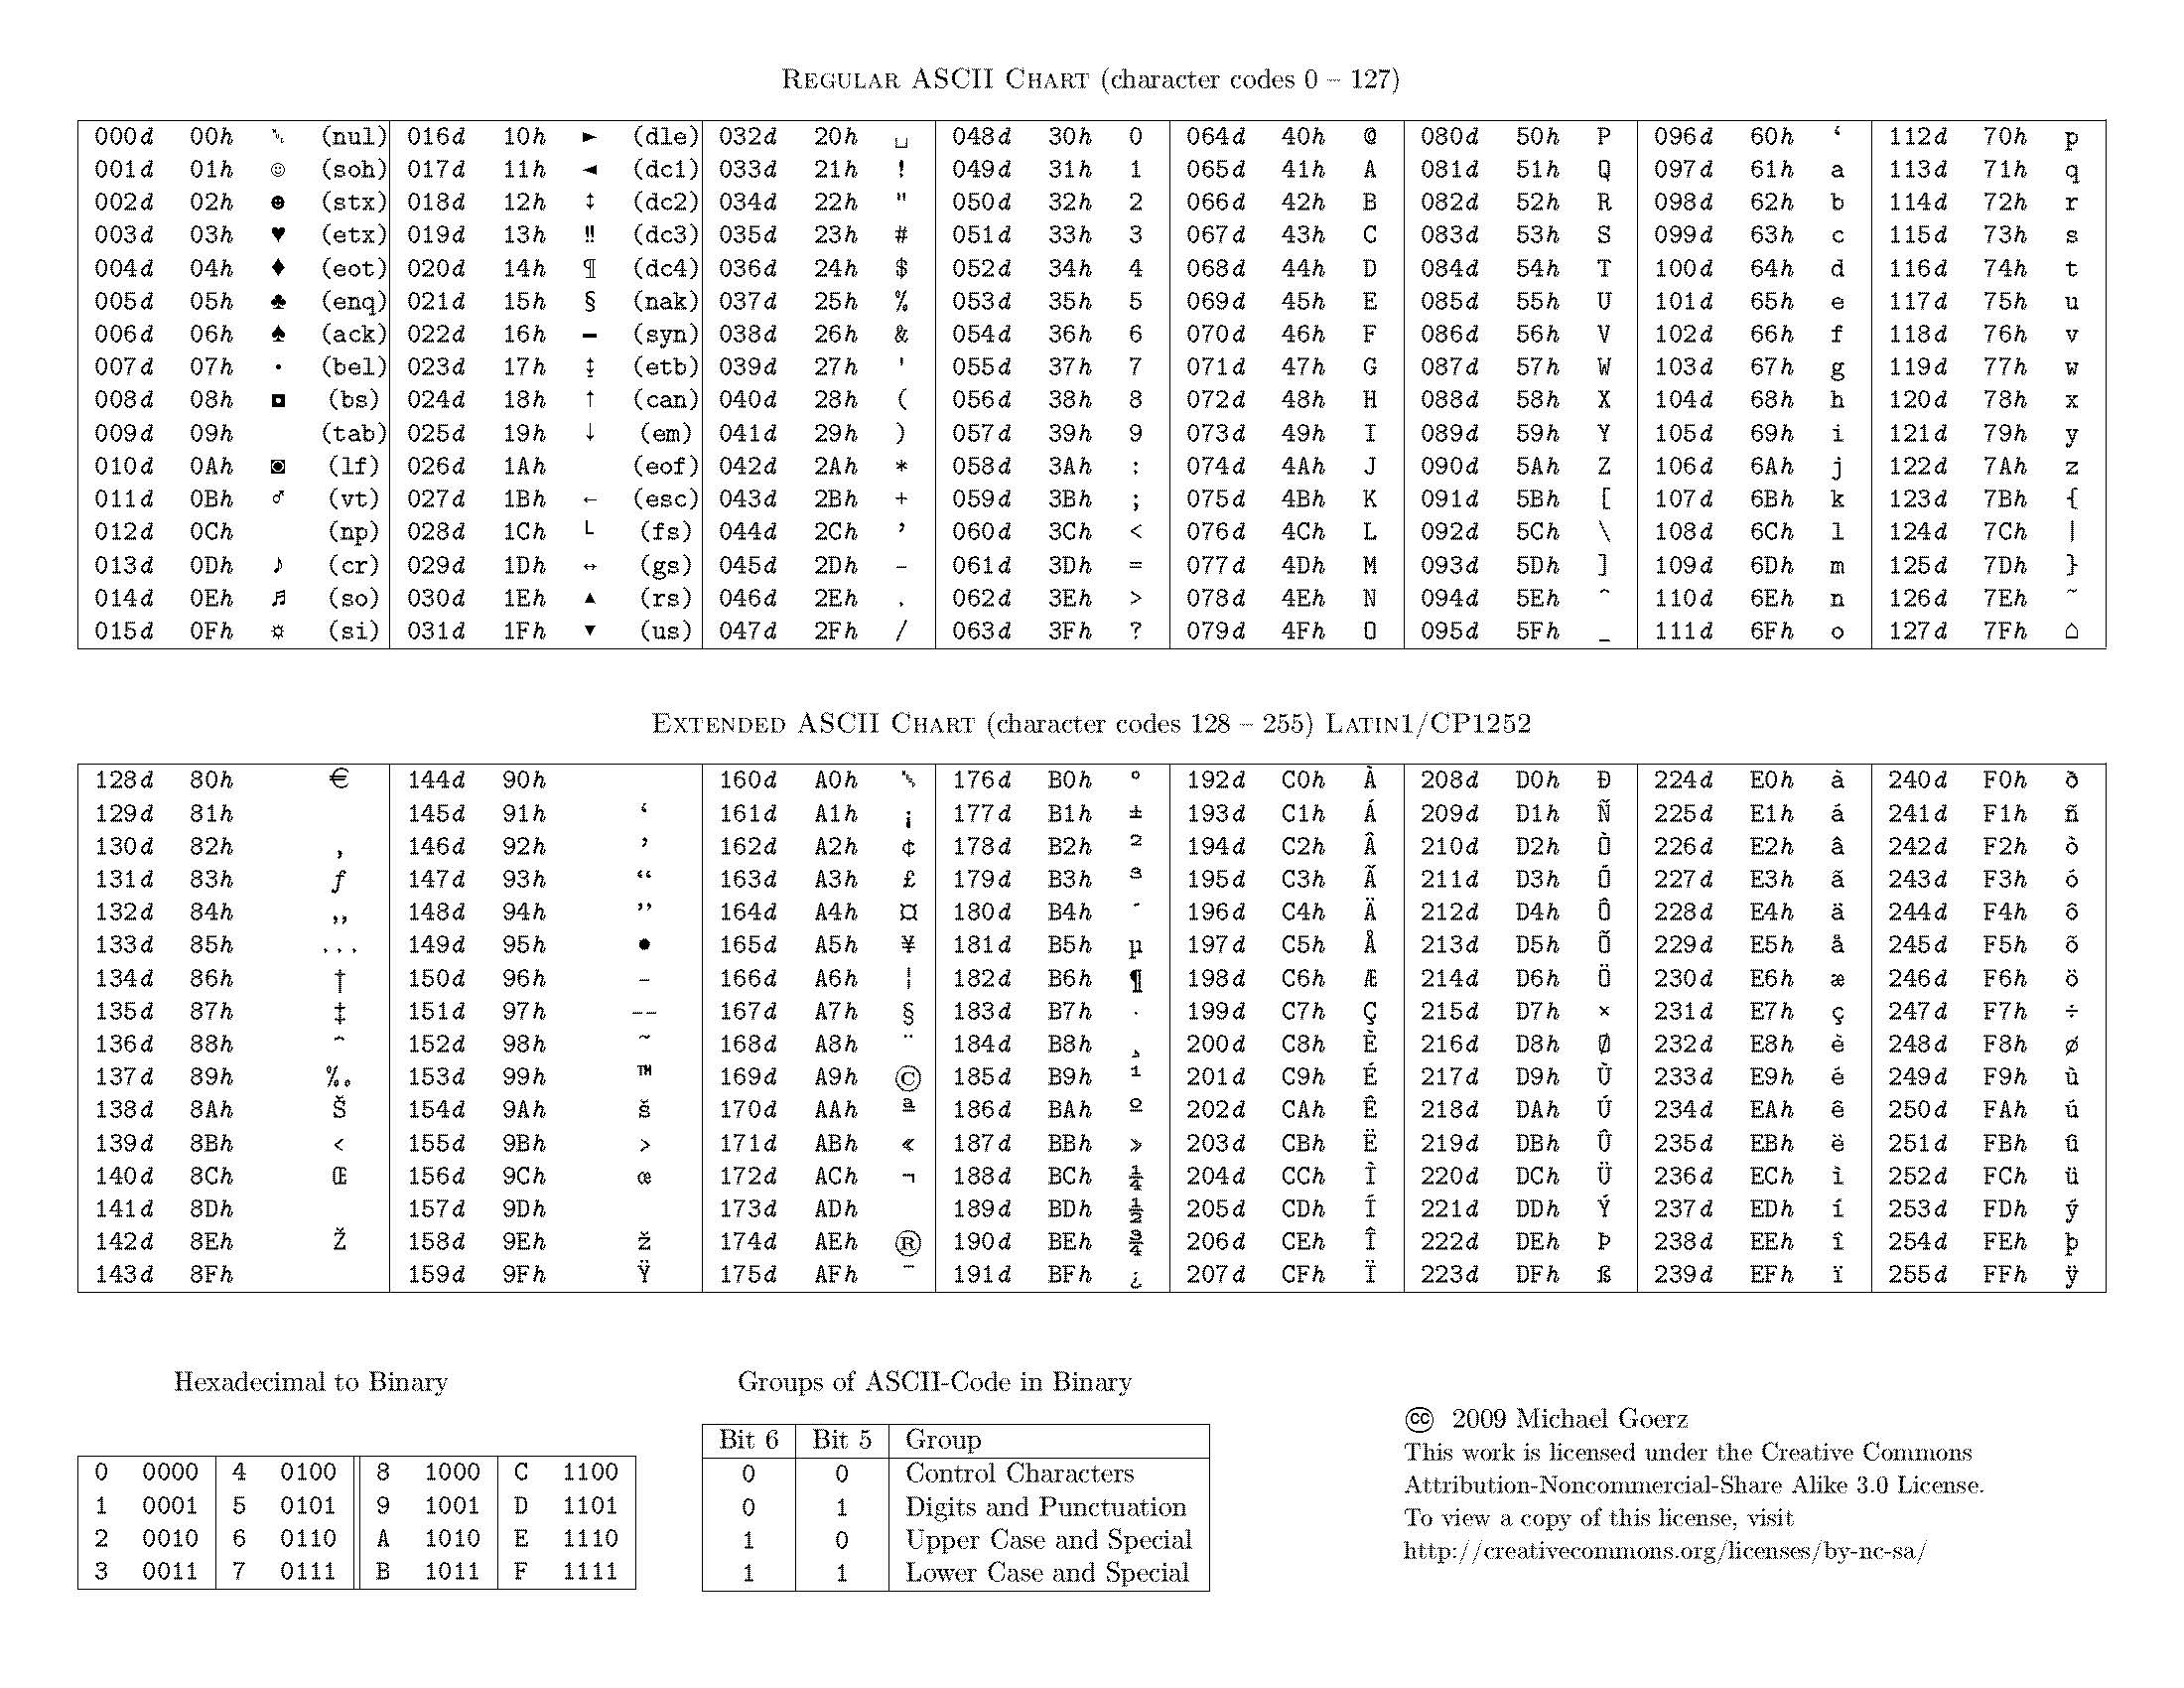
\includegraphics[width=0.8\textheight, angle=270]{ascii.jpg}
    \end{center}
\end{document}
